\documentclass[a4paper,12pt]{report}

\usepackage[utf8x]{inputenc}
\usepackage[T2A]{fontenc}
\usepackage[english, russian]{babel}
\usepackage{doxygen}


% Опционно, требует  apt-get install scalable-cyrfonts.*
% и удаления одной строчки в cyrtimes.sty
% Сточку не удалять!
% \usepackage{cyrtimes}

% Картнки и tikz
\usepackage{graphicx}
\usepackage{tikz}
\usetikzlibrary{snakes,arrows,shapes}


% Увы, поля придётся уменьшить из-за листингов.
\topmargin -1cm
\oddsidemargin -0.5cm
\evensidemargin -0.5cm
\textwidth 17cm
\textheight 24cm

\sloppy



% Оглавление в PDF
\usepackage[
bookmarks=true,
colorlinks=true, linkcolor=black, anchorcolor=black, citecolor=black, menucolor=black,filecolor=black, urlcolor=black,
unicode=true
]{hyperref}

% Для исходного кода в тексте
% \newcommand{\Code}[1]{\texttt{#1}}

% Некоторая русификация.
% \usepackage{misccorr} % Oh shi^W^W, оно не работает с report.
\usepackage{indentfirst}
\renewcommand{\labelitemi}{\normalfont\bfseries{--}}

% На дворе XXI век, но пакет listings всё ещё не пашет с русскими комментариями!

% Пакет listings для простой вставки исходников
% \usepackage{listings}
% Параметры оформления
% \lstset{
% showspaces=false,
% showtabs=false,
% frame=single,
% tabsize=4,
% basicstyle=\ttfamily,
% identifierstyle=\ttfamily,
% commentstyle=\itshape,
% stringstyle=\ttfamily,
% keywordstyle=\ttfamily,
% breaklines=true
% }
% Русский в комментариях.
% \lstset{escapebegin=\begin{cyr},escapeend=\end{cyr}}



% А это взято из файла, сгенерённого doxygen
%\usepackage{calc}
%\usepackage{array}
%\newenvironment{Code}
%{\footnotesize}
%{\normalsize}
%\newcommand{\doxyref}[3]{\textbf{#1} (\textnormal{#2}\,\pageref{#3})}
%\newenvironment{DocInclude}
%{\footnotesize}
%{\normalsize}
%\newenvironment{VerbInclude}
%{\footnotesize}
%{\normalsize}
%\newenvironment{Image}
%{\begin{figure}[H]}
%{\end{figure}}
%\newenvironment{ImageNoCaption}{}{}
%\newenvironment{CompactList}
%{\begin{list}{}{
%  \setlength{\leftmargin}{0.5cm}
%  \setlength{\itemsep}{0pt}
%  \setlength{\parsep}{0pt}
%  \setlength{\topsep}{0pt}
%  \renewcommand{\makelabel}{\hfill}}}
%{\end{list}}
%\newenvironment{CompactItemize}
%{
%  \begin{itemize}
%  \setlength{\itemsep}{-3pt}
%  \setlength{\parsep}{0pt}
%  \setlength{\topsep}{0pt}
%  \setlength{\partopsep}{0pt}
%}
%{\end{itemize}}
%\newcommand{\PBS}[1]{\let\temp=\\#1\let\\=\temp}
%\newlength{\tmplength}
%\newenvironment{TabularC}[1]
%{
%\setlength{\tmplength}
%     {\linewidth/(#1)-\tabcolsep*2-\arrayrulewidth*(#1+1)/(#1)}
%      \par\begin{tabular*}{\linewidth}
%             {*{#1}{|>{\PBS\raggedright\hspace{0pt}}p{\the\tmplength}}|}
%}
%{\end{tabular*}\par}
%\newcommand{\entrylabel}[1]{
%   {\parbox[b]{\labelwidth-4pt}{\makebox[0pt][l]{\textbf{#1}}\vspace{1.5\baselineskip}}}}
%\newenvironment{Desc}
%{\begin{list}{}
%  {
%    \settowidth{\labelwidth}{40pt}
%    \setlength{\leftmargin}{\labelwidth}
%    \setlength{\parsep}{0pt}
%    \setlength{\itemsep}{-4pt}
%    \renewcommand{\makelabel}{\entrylabel}
%  }
%}
%{\end{list}}
%\newenvironment{Indent}
%  {\begin{list}{}{\setlength{\leftmargin}{0.5cm}}
%      \item[]\ignorespaces}
%  {\unskip\end{list}}
%


\title{Расчётно-пояснительная записка \\  к курсовой работе на тему: \\ "Разработка серверной части  MTA SMTP" \\ по курсу: Протоколы вычислительных сетей}
\author{Жаровой Наталии Александровны\newline}

\begin{document}

\maketitle

\tableofcontents

\addcontentsline{toc}{chapter}{Введение}
\chapter*{Введение}

Цель работы: разработка серверной части MTA SMTP.

Основные задачи: проектирование, реализация и тестирование почтового сервера
(MTA).

Основные требования к серверу: 
\begin{itemize}
\item Сервер должен подерживать команды HELO и EHLO, MAIL, RCPT, DATA, RSET,
QUIT, VERIFY протокола SMTP. 
\item Серверу следует реализовать только указанные команды. VERIFY должен при этом
выдавать всегда ошибку.
\end{itemize}

Задание 5 варианта: poll и рабочие потоки. Журналирование в
отдельном потоке.

%Это~-- шаблон отчёта (вот как оформляется длинное тире, перед котрым идёт неразрывный пробел).
%
%Нумерованный список выглядит следующим образом.
%\begin{enumerate}
%\item Первый элемент.
%\item Второй элемент.
%\end{enumerate}

\chapter{Аналитический раздел}

\section{Протокол SMTP}

SMTP (англ. \textbf{S}imple \textbf{M}ail \textbf{T}ransfer \textbf{P}rotocol) ~-- это широко используемый сетевой протокол, предназначенный для передачи писем электронной почты в сетях TCP/IP. SMTP впервые был описан в RFC 821 (1982 год), а последнее обновление описано в RFC 5321 (2008 год) и включает масштабируемое расширение протокола — ESMTP (Extended SMTP). В настоящее время под протоколом SMTP подразумеваются и его расширения. Протокол SMTP предназначен для передачи исходящей почты с использованием порта TCP 25.

Взаимодействие в рамках SMTP строится по принципу двусторонней связи, которая устанавливается между отправителем и получателем почтового сообщения. При этом отправитель инициирует соединение и посылает запросы, а получатель - отвечает на эти запросы. Таким образом, отправитель выступает в роли клиента, а получатель - сервера.


\subsection{Базовые команды SMTP}

Каждая команда SMTP начинается с ключевого слова – названия команды, указывающего какую операцию хочет произвести клиент. За ним могут следовать параметры, отделенные пробелом. Конец строк в протоколе SMTP обозначается последовательностью символов "возврат каретки"\ (\textbackslash r) и "перевод строки"\ (\textbackslash n) - эта последовательность обозначается CRLF. Сервер начинает выполнение команды только получив от клиента строку, завершающуюся последовательностью CRLF. 

Обычный ответ SMTP сервера на команды клиента состоит из номера ответа, за которым через пробел следует дополнительный текст. Номер ответа служит индикатором состояния сервера и делится на четыре группы:
\begin{itemize}
    \item Команда выполнена успешно (код 2xx);
    \item Промежуточный положительный результат. Команда принята, но сервер ожидает от клиента дополнительные данные для завершения операции (код 3xx);
    \item Исполнение команды временно невозможно. Команда не может быть выполнена, но проблема может быть устранена (код 4xx);
    \item Исполнение команды невозможно (код 5xx).
\end{itemize}

Если ответ состоит из нескольких строк, то каждая из них начинается номером, который отделяется от сопровождающего текста не пробелом, а символом "минус"\ (-). В последней строке номер отделяется от текста пробелом. Каждая строка ответа, как и строки команд, заканчивается последовательностью CRLF.

Ниже представлен список базовых SMTP-команд:
\begin{itemize}
    \item EHLO доменное\_имя\_клиента CRLF - Открывает ESMTP сессию. В ответ на эту команду сервер сообщает, готов ли он к продолжению диалога.
    \item HELO доменное\_имя\_клиента CRLF - Открывает SMTP сессию. В RFC 2821 рекомендуется использовать команду HELO, только если программное обеспечение не поддерживает команду EHLO. Отличие этой команды только в том, что она делает невозможным использование расширений ESMTP. Передача почты возможна только после выполнения одной из двух перечисленных выше команд.
    \item MAIL FROM: <адрес\_отправителя> CRLF - Сообщает адрес отправителя письма. Для каждого письма команда MAIL должна быть выполнена только один раз. Адрес может быть оставлен пустым: <>. Команда MAIL может быть выполнена только после успешного выполнения команды EHLO или HELO.
    \item RCPT TO: <адрес\_получателя> CRLF - Сообщает адрес получателя письма. Доставка сообщения возможна, только если указан хотя бы один адрес получателя. Команда RCPT принимает в качестве аргумента только один адрес. Если нужно послать письмо большему числу адресатов, то команду RCPT следует повторять для каждого. Команда RCPT может быть выполнена только после успешного выполнения команды MAIL.
    \item DATA CRLF - Определяет начало письма. C помощью этой команды серверу передается текст сообщения, состоящий из заголовка и отделенного от него пустой строкой тела сообщения. В ответ на правильно введенную команду DATA сервер сообщает о готовности к приему или об ошибке, если прием сообщения невозможен. Передача самого сообщения заканчивается строкой, состоящей из одной точки. Эта строка не является частью сообщения и удаляется на приемной стороне. Команда DATA может быть выполнена только после успешного выполнения хотя бы одной команды RCPT.
    \item RSET CRLF - Сброс SMTP соединения. Команда RSET аннулирует все переданные до нее на сервер данные.
    \item VRFY CRLF - Проверяет наличия указанного в качестве аргумента почтового ящика.
    \item QUIT CRLF - Закрыть SMTP сессию. Командой QUIT клиент заканчивает диалог с сервером. Сервер посылает подтверждение и закрывает соединение. Получив это подтверждение, клиент тоже прекращает связь.
\end{itemize}

\section{Плюсы и минусы использования многопоточного подхода обработки подключений при помощи мультиплексирования и системного вызова poll()}

В рамках задания необходимо реализовать серверную часть MTA SMTP с использованием системного вызова \texttt{poll()} в нескольких рабочих процессов. К плюсам данного подхода можно отнести:
\begin{itemize}
    \item Возможность распределения нагрузки по нескольким потокам
    \item системный вызов \texttt{poll()} подходит для большинства задач, не имеет ограничения на количество отслеживаемых дескрипторов, как в \texttt{select()}
\end{itemize}

К недостаткам данного подхода относятся:
\begin{itemize}
    \item Системный вызов \texttt{poll()} сложнее в использовании, чем \texttt{select()}
    \item Создание отдельных потоков - дополнительные расходы и нагрузка на систему, однако использование пула потоков позволяет значительно снизить нагрузку
\end{itemize}

\section{Сущности предметной области}

Сущности предметной области предствалены на ER-диаграмме (рис \ref{fig:er}).

\begin{figure}
\centering
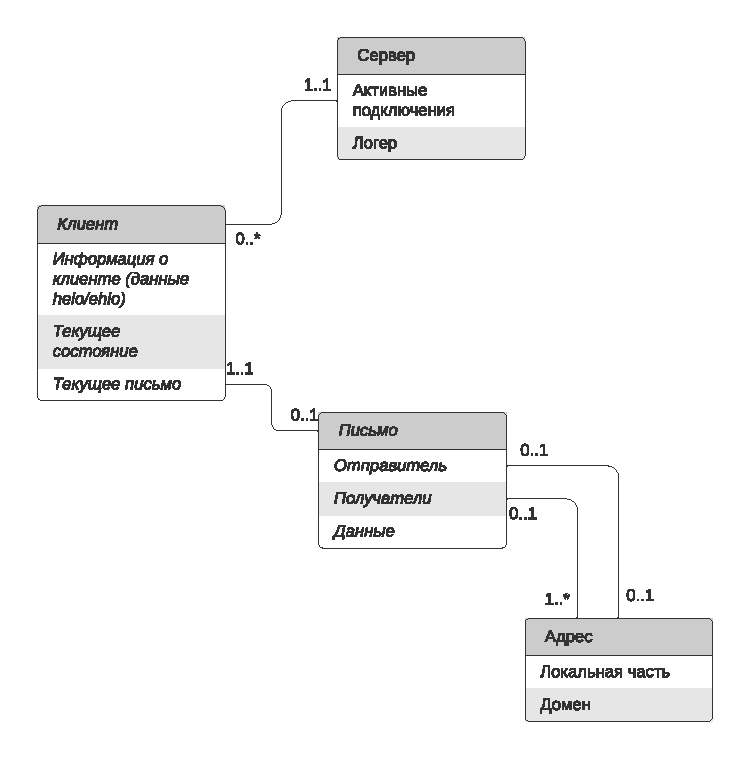
\includegraphics[width=\textwidth]{diagramms/er.pdf}
\caption{ER-диаграмма предметной области}
\label{fig:er}
\end{figure}

\chapter{Конструкторский раздел}

\section{Конечный автомат состояний сервера}

%Рис.~\ref{fig:fsm} нагенерил самодельный \textit{fsm2dot} из \textit{autogen} и \textit{dot2tex} на пару \textit{dot}. Никто не мешает изменить параметры типа \textit{rankdir} прямо в \textit{fsm2dot}, если он будет лучше смотреться, например, сверху-вниз.

На рис.~\ref{fig:fsm} изображен конечный автомат состояний серверной части MTA SMTP. 

\begin{figure}
\centering
\includegraphics[width=\textwidth]{include/client_def_dot.pdf}
\caption{Состояния сервера}
\label{fig:fsm}
\end{figure}

\section{Синтаксис команд протокола}

\subsection{Команды протокола}
\begin{description}
\item[Команда HELO]
\input{include/re_helo_re.tex}
\item[Команда EHLO]
\input{include/re_ehlo_re.tex}
\item[Команда MAIL]
\input{include/re_mail_re.tex}
\item[Команда RCPT]
\input{include/re_rcpt_re.tex}
\item[Команда DATA]
\input{include/re_data_re.tex}
\item[Команда VRFY]
\input{include/re_vrfy_re.tex}
\item[Команда RSET]
\input{include/re_rset_re.tex}
\item[Команда QUIT]
\input{include/re_quit_re.tex}
\end{description}

\subsection{ Основные вспомогательные выражения, используемые для описания команд протокола}
\begin{description}
\item[RE\_DOMAIN]
\input{include/re_domain_re.tex}
\item[RE\_SUB\_DOMAIN]
\input{include/re_sub_domain_re.tex}
\item[RE\_FORWARD\_PATH]
\input{include/re_forward_path_re.tex}
\item[RE\_REVERSE\_PATH]
\input{include/re_reverse_path_re.tex}
\item[RE\_PATH]
\input{include/re_path_re.tex}
\item[RE\_MAILBOX]
\input{include/re_mailbox_re.tex}
\end{description}


%Для грамматики можно использовать вставку из файла и оформление \textbackslash{}begin\{verbatim\} и \textbackslash{}end\{verbatim\} или пакет \textit{listings}\footnote{На дворе XXI век, но пакет \textit{listings} всё ещё не пашет с русскими комментариями без бубна, и лично я его пока не победил.}.

\section{Параметры командной строки}

%Для примера воспользуемся автоматической вставкой файла описания параметров программы (не забудьте перенести это в технологический раздел) через утилитку \textit{src2tex}.

AutoGen Definitions options;
prog-name     = server;
prog-title    = "Server";
long-opts;

flag = {
    name      = port; /* Порт, который слушает сервер */
    value     = p;              /* Краткий флаг (-p) */
    arg-type  = number;
    arg-range = 110;
    arg-range = "1024->65000";
    max       = 1;           /* Не более одного раза */
    min       = 0;          /* Опциональный параметр */
    descrip   = "Port to bind";
};

flag = {
    name      = domain;           /* Домен сервера */
    value     = d;             /* Краткий флаг (-d) */
    arg-type  = string;
    max       = 1;          /* Не более одного раза */
    min       = 0;         /* Опциональный параметр */
    descrip   = "Server domain";
};

flag = {
    name      = local_maildir;           /* Папка для локальной доставки почты */
    value     = l;             
    arg-type  = string;
    max       = 1;          /* Не более одного раза */
    min       = 0;         /* Опциональный параметр */
    descrip   = "Local maildir";
};

flag = {
    name      = client_maildir;           /* Папка для обмена почтой с клиентской частью smtp-сервера */
    value     = c;             
    arg-type  = string;
    max       = 1;          /* Не более одного раза */
    min       = 0;         /* Опциональный параметр */
    descrip   = "Client maildir";
};

flag = {
    name      = user;           /* Папка для обмена почтой с клиентской частью smtp-сервера */
    value     = u;             
    arg-type  = string;
    max       = 1;          /* Не более одного раза */
    min       = 0;         /* Опциональный параметр */
    descrip   = "User for lower priority ";
};

flag = {
    name      = backlog_queue_size;           /* Размер backlog-очереди основного сокета */
    value     = b;             
    arg-type  = number;
    arg-range = "10->150";
    max       = 1;          /* Не более одного раза */
    min       = 0;         /* Опциональный параметр */
    descrip   = "Backlog queue size of main socket";
};
% \lstset{language=C}
% \lstinputlisting{../src/checkoptn.def}

\chapter{Технологический раздел}

% Нужно отметьть, что символ <<\_>> необходимо оформлять как <<\textbackslash\_>>.

\section{Сборка программы}

Сборка программы описана в файле \textit{Makefile}, упрощённая схема представлена на рис.~\ref{fig:make}.

\begin{figure}
\centering
\includegraphics[width=0.7\textwidth]{include/Makefile_1_dot.pdf}
\caption{Сборка программы}
\label{fig:make}
\end{figure}

%\input{include/files}
%\input{include/annotated}
%\input{include/server-state_8h.tex}
%\input{include/server-re_8h.tex}
%\input{include/server-run_8h.tex}
%\input{include/server-run_8c.tex}
%\input{include/structmsg.tex}
%\input{include/structnode__t.tex}

\section{Графы вызова функций}

На рис.~\ref{fig:cflow01} показан граф вызовов основных функции.

\begin{figure}
\centering
\includegraphics[width=\textwidth]{include/cflow01_dot.pdf}
\caption{Граф вызовов, основные функции}
\label{fig:cflow01}
\end{figure}

\section{Основные структуры программы}

\input{include/structserver__info__t.tex}
\input{include/structmsg__t.tex}
\input{include/structclient__t.tex}

\input{include/structmsg__t.tex}

\section{Модульное тестирование}
Для модульного тестирования функций сервера в работе используется библиотека CUnit.
\begin{verbatim}

Run Summary:    Type  Total    Ran Passed Failed Inactive
              suites      1      1    n/a      0        0
               tests      1      1      1      0        0
             asserts     10     10     10      0      n/a

Elapsed time =    0.000 seconds
Exiting tests
\end{verbatim}

\section{Тестирование утечек памяти}

Для тестирования утечек памяти использовалась утилита valgrind.
\begin{verbatim}
==9430== HEAP SUMMARY:
==9430==     in use at exit: 0 bytes in 0 blocks
==9430==   total heap usage: 95 allocs, 95 frees, 395,991 bytes allocated
==9430== 
==9430== All heap blocks were freed -- no leaks are possible
==9430== 
==9430== ERROR SUMMARY: 0 errors from 0 contexts (suppressed: 0 from 0)

\end{verbatim}


\addcontentsline{toc}{chapter}{Выводы}
\chapter*{Выводы}

В процессе выполнения работы была написана программная реализация серверной части MTA SMTP. Был изучен протокол передачи электронной почты SMTP и способы мультиплексирования. Были закреплены и получены навыки в написании сетевых приложений на языке Си для Unix-подобных операционных систем. Было проведено тестирование и отладка разработанного приложения и в итоге по результатам проведенной работы была оформлена расчетно-пояснительная записка.



\end{document}
